%Replace Strings:
%PROJECT.TITLE
%TODO.CHANGE
%PROJECT.ABSTRACT.KEYWORDS

\documentclass[12pt, a4paper, oneside]{article}

\usepackage[utf8]{inputenc}
\usepackage[bindingoffset=1.57cm, left=2.54cm, right=2.54cm, top=2.54cm, bottom=2.54cm]{geometry}
\usepackage{mathptmx}
\usepackage{fancyhdr}
\usepackage{lipsum}
\usepackage{secdot}
\usepackage{lastpage}
\usepackage{cite}



\usepackage{graphicx}
	\graphicspath{ {images/} }

\usepackage{tocloft}
\usepackage[table,xcdraw]{xcolor}

\usepackage{floatrow}
\floatsetup[table]{capposition=top}

\linespread{1.2}
\pagestyle{fancy}
\fancyhf{} % sets both header and footer to nothing
\renewcommand{\headrulewidth}{0pt}
\rhead{ \textit{Treasure Nepal: Discover Places, Collect Treasures}}
\cfoot{\thepage}

\setlength{\parindent}{0pt}
\setlength{\parskip}{12pt}

%\frontmatter

\begin{document}

\pagenumbering{roman}
\addcontentsline{toc}{section}{Abstract}
\large
\begin{center}
	\textbf{ABSTRACT}
\end{center}

\normalsize
As we are at the brim of the Visit Nepal year 2020, the decentralization of tourism in Nepal has become absolutely necessary. Almost ninety percent of the tourists arriving Nepal visit the most popular destinations like Kathmandu, Pokhara, Chitwan and Everest, whereas the remote places like Rara Lake and Phoksundo National Park have not seen satisfactory inflow of tourists despite them being rich in natural beauty and tourism potentiality. There are still a lot of tourist destinations in Nepal that need the attention of the tourists.

Treasure Nepal is a treasure hunt application where the users travel to different places in order to collect treasures and increase their scores. The app has an integrated map that navigate the users to various tourist destinations in Nepal. The project aims to take the attention of tourists and visitors towards various tourists destinations in Nepal. The tourists need to physically reach to a place in order to collect treasures. The tourists who collect treasures at places that are remote and left behind will get higher scores than the ones who visit common popular destinations. The users can also share their scores and leaderboard status to social media. On the long run, the project sets its objective to take the tourism of Nepal to a new level.

The major deliverables proposed in the project are an Android application and a RESTful API web service.

\textbf{Keywords}: Visit Nepal 2020, Treasure hunt, Tourism\\

\break

\large
\addcontentsline{toc}{section}{Table of Contents}
\begin{center}
	\textbf{TABLE OF CONTENTS}
\end{center}


\normalsize
\setlength{\cftbeforetoctitleskip}{0pt}
\renewcommand{\contentsname}{}
\tableofcontents

\break

%\mainmatter
\cfoot{\textbf{\thepage} /  \pageref{LastPage}}

\pagenumbering{arabic}
\section{Introduction} 
Treasure Nepal is a mobile application for a treasure hunt game proposed to be tailored for tourists visiting Nepal. With the view of encouraging tourists to visit remote and unexplored part of the country, the application aims to increase the traffic of tourist in such locations as well as promote their tourism. This document looks forward to providing essential information about the needs, scope, objectives and proposed methodology of the application.

Tourism has a great potential to contribute to the Gross Domestic Product (GDP) of Nepal, but having observations at the statistics, the ratio of contribution of tourism to GDP is not satisfactory. According to Nepal Rastra Bank, the total contribution of the foreign exchange from tourism to the total Gross Domestic Product (GDP) of Nepal was 2.2\% in the year 2017/18. \cite{tourismstats}.

The Government of Nepal has taken efforts to celebrate the year 2020 officially as the Visit Nepal Year 2020. At the brim of year 2020, the authors have proposed to build a treasure hunt application specially tailored for the tourists to get their attention to unexplored and remote tourism destinations of Nepal. 

There are a few applications somehow similar to the proposed application but none of them are built for tourism purposes. Rather, they are developed only for entertainment purposes. In this context, the proposed application will distinguish itself as unique and first of the kind product in the market.

Tourism in Nepal is largely centralized to a few popular destinations. The places like Kathmandu, Pokhara, Chitwan, Annapurna area and Everest area are largely flocked by tourists while destinations like Rara Lake, Shey Phoksundo National Park or Khaptad National park struggle to get satisfactory inflow of traffic.

\subsection{Problem Statement}
The decentralisation of tourism has largely underestimated the potential and beauty of many travel destinations, specially in remote areas. As a result, these places have very low traffic of tourists. In addition, as majority of people in such places rely solely on tourism industry for their livelihood, this problem has pushed those communities even further down below the poverty line.

\subsection{Project Objectives}
The proposed project has put forward the following objectives:

\begin{itemize}
	\item To decentralize the tourism industry and encourage uniform flow of tourists at various destinations across Nepal.
	\item To promote and encourage the tourism in remote and novel destinations which otherwise are not popular or have low inflow of tourists.
	\item To explore business and economic opportunities generated by the project if taken to the production level.
\end{itemize}

\subsection{Significance of the Study}
The project proposed is significant owing to the fact that we are near the Visit Nepal Year 2020, and the proposed project will certainly be fruitful in achieving the objectives set by the Government of Nepal in the year 2020. Since the proposed idea is one of the first of its kind, it is expected that the project will reach to a significant majority of tourists that visit Nepal in 2020.

\subsection{Scope and Limitations}
In the beginning phase, the treasure hunt concept of the app will be implemented and other features are proposed to be added later gradually if possible. Such possible extensions could be addition of forex plugins, itinerary maps, guides, etc. The users will be able to collect coins from collecting the treasures, and their collection will be put in the leaderboards based on the user's local location as well as country-wise and globally. The application will have an integrated map, which enlists the tourist destinations in the locality of tourist's current location. The application will also be connected to third party social networking platforms like Facebook, Twitter, etc. so that the users can share their collection and score. 

The scores of the treasures will be calculated based on the factors like the difficulty to reach the destination, its novelty, potentiality to attract new tourists and other similar criteria. The users will receive more amount of score when visiting rural and novel places than visiting urban and frequently visited places.

The following are the limitations of the project that are realized:
\begin{itemize}
 	\item The application will be built on Android platform in the beginning and later extended to iOS, but not for other mobile operating systems like Blackberry and Windows.
	\item QR code scanning will be the method of collection of treasures and no other validation architecture will be used except for the check of location when the user scans the QR.
 \end{itemize}

\break
\section{Literature Review}
This section consists description of the literature study performed during the development of this proposal.

\subsection{Visit Nepal 2020}
The Visit Nepal 2020 project was officially introduced by Nepal Tourism Board (NTB) in 2015. The project aims to bring two million tourists in Nepal during the year 2020 \cite{visitnepal}. The slogan of Visit Nepal 2020 has been translated to more than ten different languages. The board also is planning to train ten thousand people to provide quality service to the tourists. 

\subsection{Attractions in Nepal}
The major itineraries of the tourists visiting Nepal include mountaineering, trekking, religious pilgrimages and holiday spending. The northern part of Nepal has the mountain range with highest elevation in the world, called as the Himalayas \cite{himalayas}. These mountains serve as a destination for the tourists seeking mountaineering as welll as trekking. The famous trekking destinations in Nepal are Everest Base Camp, Annapurna Circuit and Langtang Trekking Route \cite{trekkingroutes}. Other attractions include various lakes, the famous of which are Tilicho Lake, Rara Lake, Phewa Lake and Gosaikunda.

Nepal is also rich in biodiversity. Currently there are 12 national parks, 1 wildlife reserve, 6 conservation areas, 1 hunting reserve and 10 Ramsar sites as the protected areas of Nepal \cite{protectedareas}. Among them, Chitawan National Park is the most popular one. A lot of tourists visit these areas for the purpose of jungle safari and animal sports.

Nepal is rich in cultural diversity too. A large portion of the tourist inflow in Nepal occurs for religious and pilgrimage purposes. In recent years, the various communities have incorporated home stay programmes to host tourists in their home and offer their cultural courtesy, which has sent setup good environment for the cultural tourism in Nepal. The festivals like Dashain, Lhosar, Chhath, Gai Jatra, Buddha Jayanti, etc. are some of the most popular festivals of Nepal.

\subsection{Existing Similar Appilcations}
There are several treasure hunt applications available in the application stores developed for entertainment purposes. Some of them are GooseChase, Locandy, Huntzz, Scavify and Geocaching \cite{similarapps}. The proposed application distinguishes itself from these applications due to its focus on the tourism industry. The available applications are developed only for entertainment purposes. Also, the users themselves have to set treasures and spots and enter them into the application to create a challenge and then challenge someone else to find and collect them. In contrast, the users of the proposed application are already provided with the treasures and they don't actively take participation in creating one.

\subsection{Challenges}
One of the major challenges realized is the validation of the collection of treasures by the users. If only QR code is used for validating that a tourist has in fact reached a destination, there is a high chance that the QR codes get shared among people and people will remotely validate themselves having gone to a place and collected a treasure just by scanning the photo of the QR from a remote location. A countermeasure that can be used is to add actual location data from the user's phone's GPS sensor as an additional parameter for validation. A treasure is only considered to be collected if a user scans the QR from within a specific distance from the actual treasure location.

GPS spoofing is one of the major challenges for any system that has used GPS for the validation. GPS spoofing is the process of modifying a GPS receiver unit so that it broadcasts incorrect GPS signal. Some countermeasures to tackle GPS spoofing are monitoring absolute as well as relative GPS signal strength; checking time intervals and performing comparision; and performing sanity checks \cite{gpsspoofmeasures}.

\break
\section{Proposed Methodology}
This section describes the methodology that is proposed to be followed during the development of the project.

\subsection{Proposed Software Development Life Cycle}
The project will be developed as per the waterfall model of software development life cycle as depicted in Figure \ref{fig:sdlc}. The reason for choosing this model is the lack of sufficient time duration for agile and iterative methods, as well as very low chances of the changes of requirements in the process of development. 

\begin{figure}[h]
	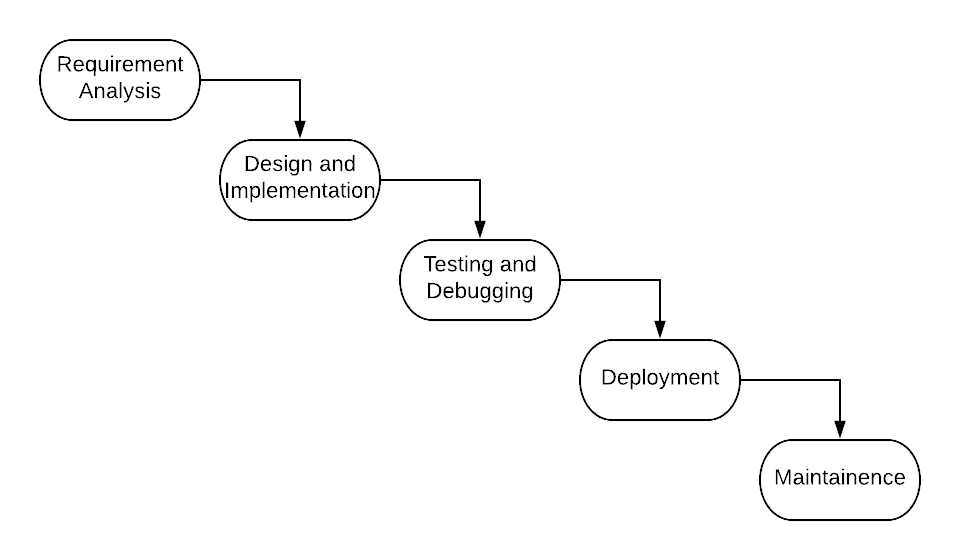
\includegraphics[width=\linewidth]{sdlc}
	\centering
	\caption{Proposed software development life cycle}
	\label{fig:sdlc}
\end{figure}

The life cycle begins when the team collects and evaluates the requirements that will be expected from the application. The design and implementation phase will be to design and build both API services and client applications. By the end of this phase, a minimal viable product (MVP) will already have been constructed. In the testing and debugging phases, the quality control methods will be applied to both API and application. Finally, the application will be deployed to the Amazon Web Services at the end of the deployment phase. However, there might be slight modifications in the original waterfall model where the design and implementation may be changed slightly after the testing phase if seen reasonable.

\subsection{Technical Architecture}
The application will be built upon the client-server web architecture, as illustrated in Figure \ref{fig:arch}.

\begin{figure}[h]
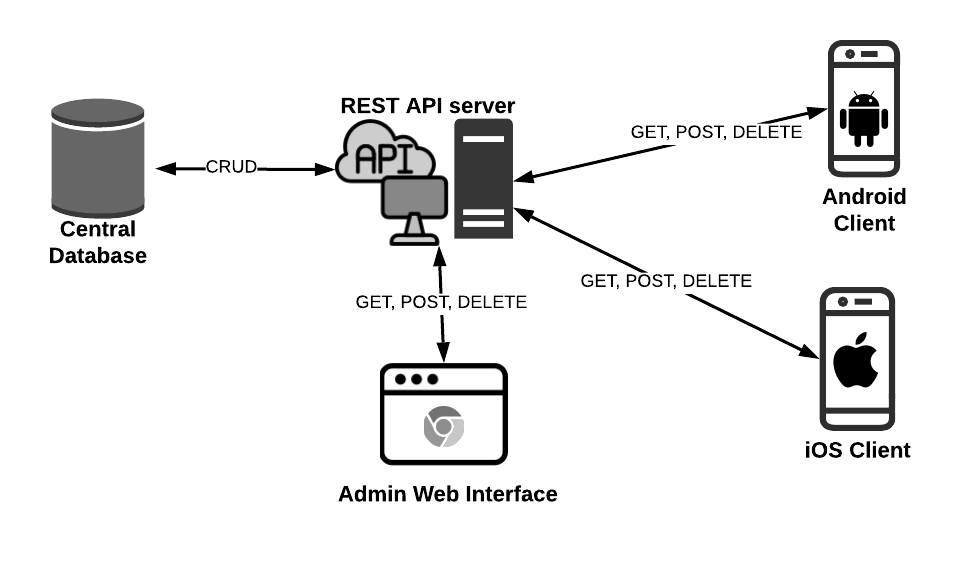
\includegraphics[width=\linewidth]{architecture}
\centering
\caption{Proposed architecture of the application}
\label{fig:arch}
\end{figure}

At the heart of the architecture lies the RESTful web service which communicates directly with the central database where all the data is stored. The mobile applications as well as the admin web interface do not access the database directly, but via the API service. The clients send HTTP requests like GET, POST and DELETE, while the API service processes those requests and return the data in JSON format.

\subsection{Proposed Technologies}
Table \ref{table:tech} consists of the major technologies that are proposed to be used during development and deployment of the application.

\renewcommand{\arraystretch}{1.5}
\begin{table}[]
\begin{tabular}{|l|l|}
\hline
\rowcolor[HTML]{C0C0C0} 
\textbf{Subject}    & \textbf{Proposed Technology} \\ \hline
Backend Database            & MySQL                        \\ \hline
REST API Service    & Django REST Framework        \\ \hline
Android Client  & React Native                 \\ \hline
Admin Web Interface & Django Framework             \\ \hline
Deployment Platform & Amazon Web Services (AWS)    \\ \hline
Documentation & LaTeX \\ \hline
\end{tabular}
\caption{Technologies proposed to be used}
\label{table:tech}
\end{table}


\pagebreak
. \pagebreak
\section{Proposed Deliverables}
The following will be the major deliverables that will be produced at the end of this project.

\subsection{RESTful API service}
There will be a running instance of RESTful API service developed and deployed at the end of the project. This API will be responsible for communicating between the client applications and the central database server.

\subsection{Android client application}
The application will be developed integrating all the features proposed earlier. The users will be able to use the application to scan QR codes at different travel destinations which will reward them with scores in their accounts. An interactive map will be integrated with the application that shows the treasures installed at various tourist destinations near to the tourist's current location. The application will also be integrated with social networking platforms like Facebook, Twitter, Instagram etc. so the tourists can share their scores publicly to their friends and acquaintances. 

\break
\section{Project Task and Time Schedule}
The working time period for the project is three months. The project will be completed by the end of the spring semester as per the requirements of the university. The major task division among the team members is mentioned in Table \ref{table:taskdiv}.

\begin{table}[h!]
\begin{tabular}{|l|l|}
\hline
\rowcolor[HTML]{C0C0C0} 
\textbf{Team Member} & \textbf{Assigned Tasks}                                                                                                                     \\ \hline
Bikalpa Dhakal       & \begin{tabular}[c]{@{}l@{}} Project Management\\Android Application Development\\ Deployment to AWS\end{tabular} \\ \hline
Avinash Shreshtha   & \begin{tabular}[c]{@{}l@{}}API Development\\ Data Management\\ Project Documentation\end{tabular}                                           \\ \hline
\end{tabular}
\caption{Division of tasks among project team members}
\label{table:taskdiv}
\end{table}

The time schedule proposed for the development of the project is illustrated in Figure \ref{fig:schedule}.

\begin{figure}[h!]
	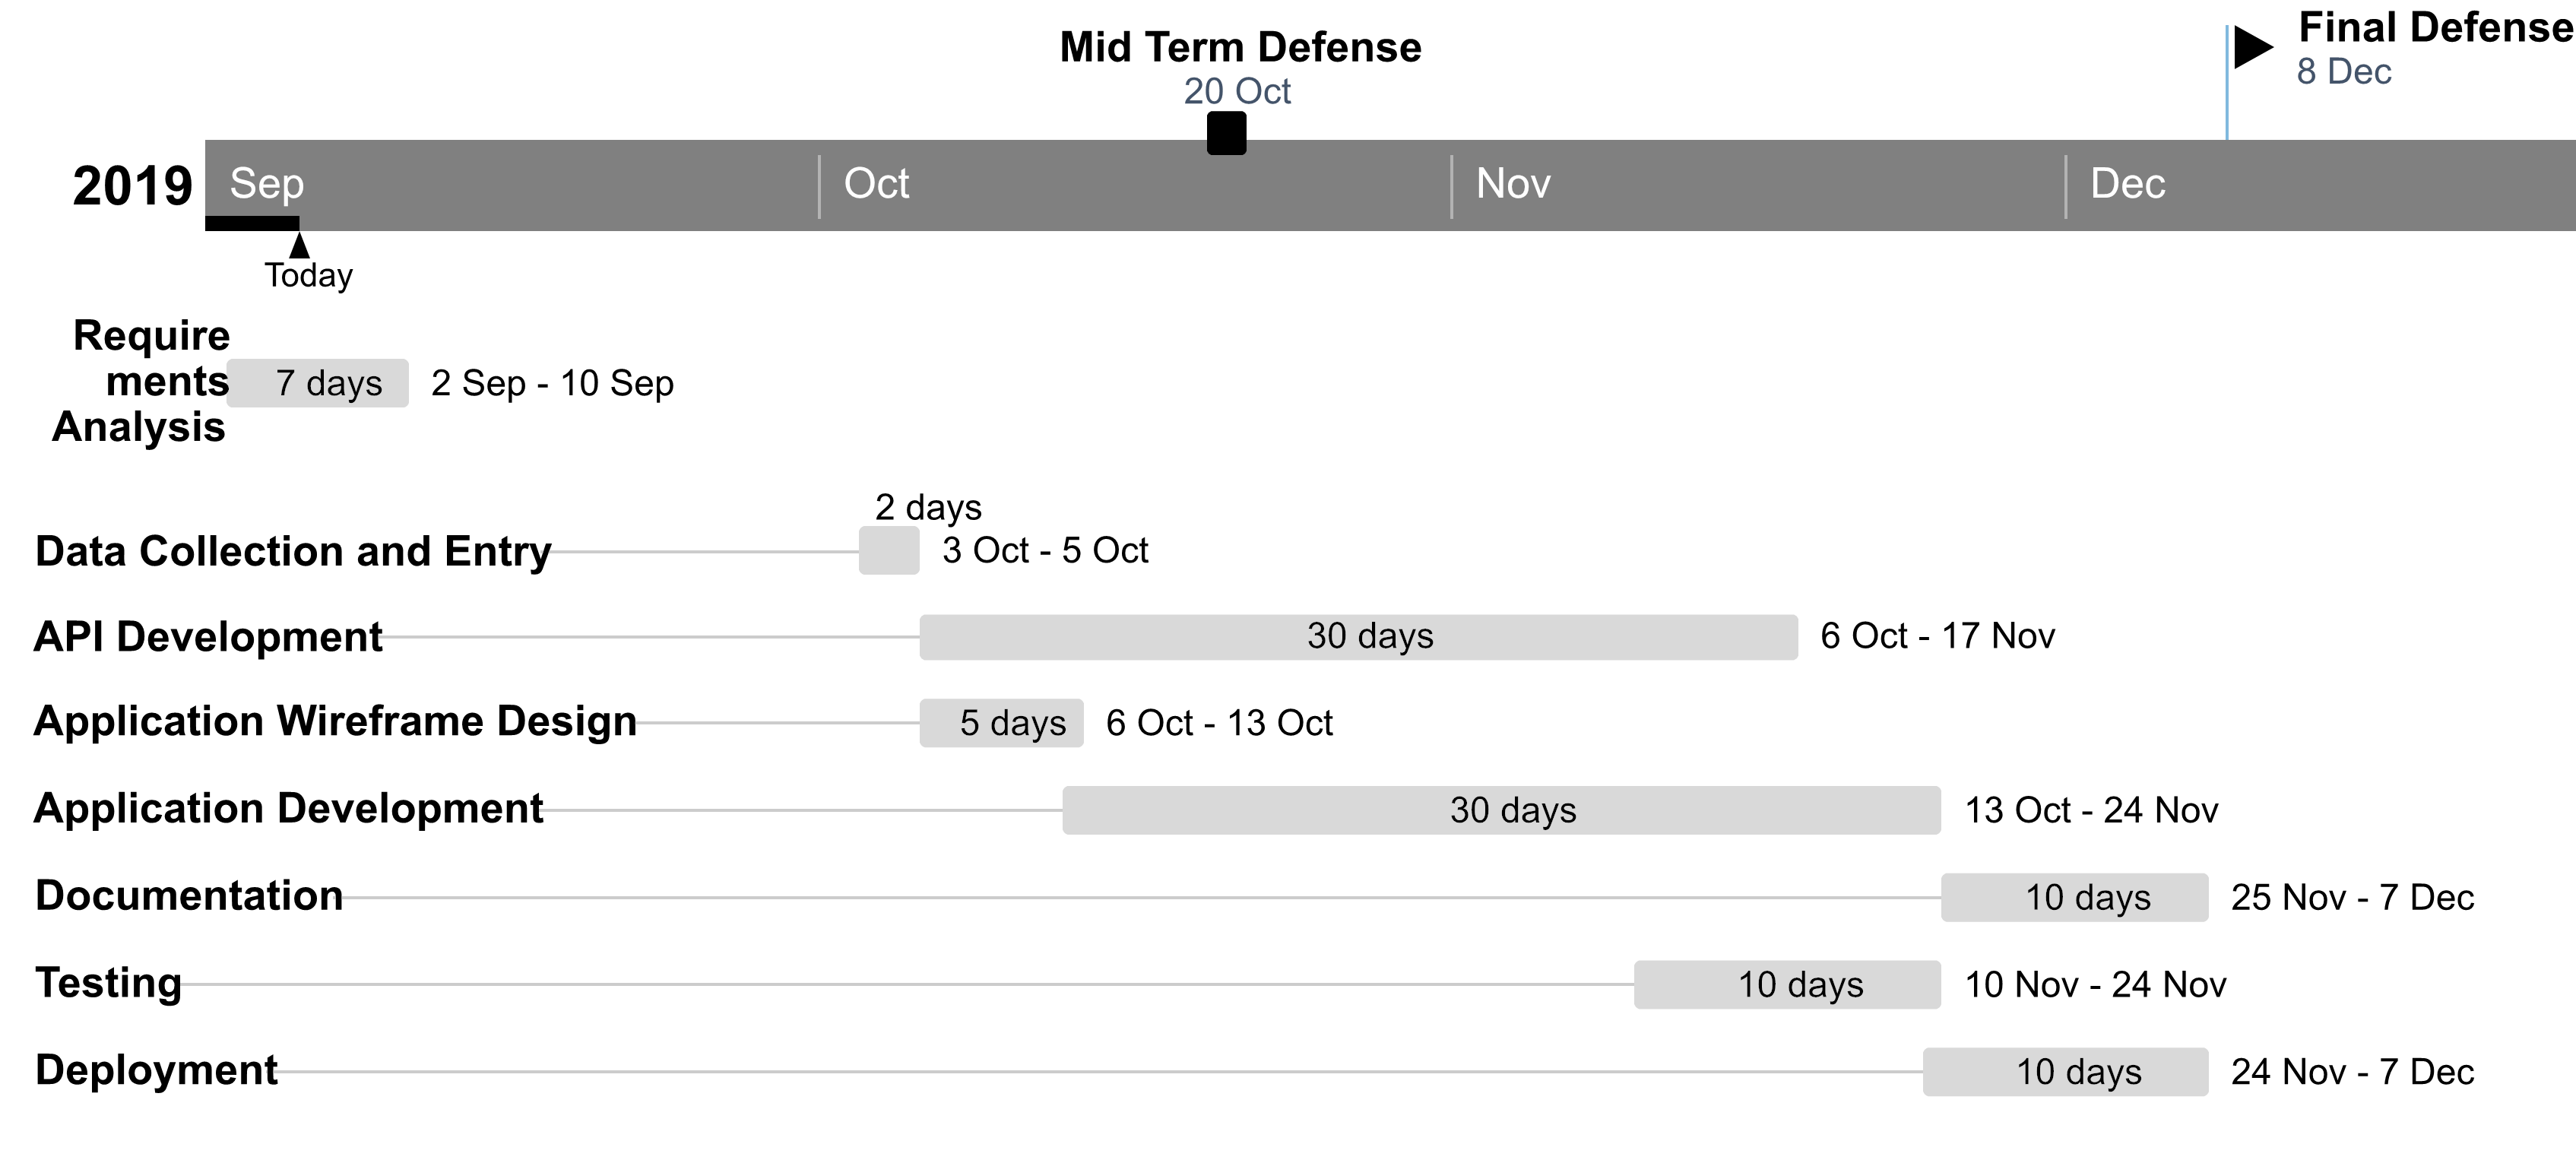
\includegraphics[width=\linewidth]{schedule}
	\centering
	\caption{Proposed project schedule}
	\label{fig:schedule}
\end{figure}



\break
\addcontentsline{toc}{section}{References}
\bibliography{references}
\bibliographystyle{ieeetran}

\end{document}

%\break
%\section{Proposed Performance Analysis Methodology}
%The performance analysis of the deliverables will be performed according to the popular Top Down Methodology. The main idea in this method is to analyse and address the higher order performance issues at first, then follow the lead upto the lower levels of details if needed \cite{tdmethod}. This methodology is proposed to be followed because it largely reduces the time and cost of assessing the performance since not every modules and sections of the project need to be analyzed at a deeper level.
%
%The final evaluation of the project will be performed by the project evaluation team designated by the college administration.
